\subsection{بخش پ}
در این بخش به بررسی تاثیر
\lr{T}
بر فاصله‌ ازدست‌دهی و تلاش کنترلی پرداخته شده است.
\begin{figure}[H]
	\centering
	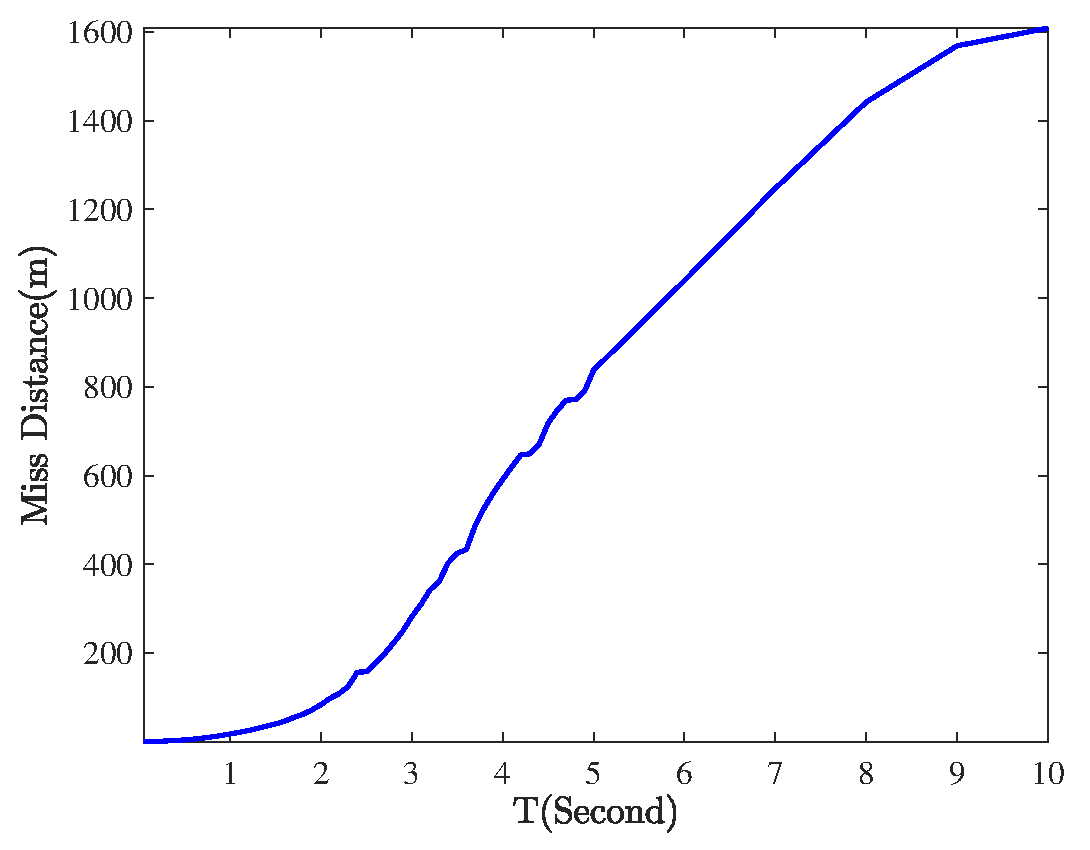
\includegraphics[width=.75\linewidth]{../Figure/Q1/c/MD}
	\caption{فاصله ازدست‌دهی برای مقادیر مختلف \lr{T}}
\end{figure}

\begin{figure}[H]
	\centering
	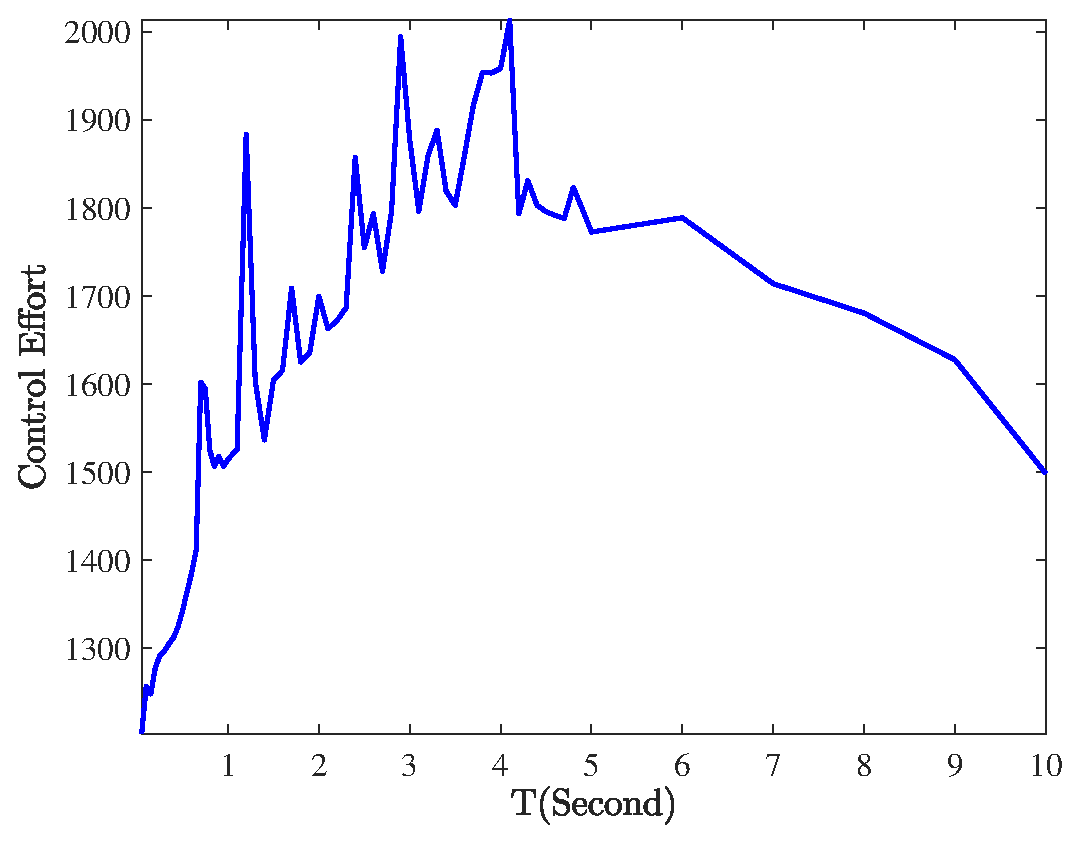
\includegraphics[width=.75\linewidth]{../Figure/Q1/c/CE}
	\caption{تلاش کنترلی برای مقادیر مختلف \lr{T}}
\end{figure}

بر اساس نتایج بالا با افزایش \lr{T} فاصله ازدست‌دهی زیاد می‌شود و یر اساس میزان دقت می‌توان محدوده قابل قبول را بدست آورد. در اینجا، برای مقادیر کمتر از ۱ نتایج معقولی دارد و می‌توان ار آن استفاده کرد. از طرفی، تلاش کنترلی با افزایش \lr{T} ابتدا افزایش سپس کاهش می‌یابد.